\documentclass[landscape]{foils}
\usepackage[pdftex]{color}
\usepackage[pdftex]{graphicx}
\usepackage{eso-pic}
\usepackage[top=2cm, bottom=2cm, outer=0cm, inner=0cm]{geometry}
\usepackage{listings}
\usepackage{amsmath}


\DeclareMathOperator{\sign}{sign}

% colors
\definecolor{DarkRed}{rgb}{0.5,0.0,0.0}
\definecolor{DarkBlue}{rgb}{0.0,0.0,0.35}
\definecolor{DarkGreen}{rgb}{0.0,0.6,0.00}
\definecolor{Orange}{rgb}{0.70,0.30,0.0}
\definecolor{Magenta}{rgb}{0.8,0.0,0.8}
\definecolor{DarkGray}{rgb}{0.3,0.3,0.3}
\def\red{\color{red}} 
\def\darkred{\color{DarkRed}} 
\def\blue{\color{DarkBlue}} 
\def\green{\color{DarkGreen}} 
\def\orange{\color{Orange}}
\def\magenta{\color{Magenta}}
\def\black{\color{black}}
\def\gray{\color{DarkGray}}

% sizes, footer and headers
\textwidth = 26truecm
\textheight = 18truecm
\topmargin =-2 cm
\oddsidemargin -1.5cm
\rightfooter{}
\MyLogo{\darkred {\bf QE-2019}: Summer School on Advanced Materials
  and Molecular Modelling}
%
\def\indent{\hspace*{1cm}}
\def\prompt{\texttt{\$~}}
\def\exec#1{\indent\prompt\code{#1}}
\def\codeline#1{\indent\code{#1}}
\parindent 0pt

% alias for slides header
\def\Head#1{\foilhead{\red #1 \vskip -1cm} \medskip\hrule\medskip}
\def\head#1{\foilhead{\red #1 \vskip -1cm}}

% aliases for codes, files, namelists, etc.
\def\codecolor{\green}
\def\cardcolor{\orange}
\def\code#1{\texttt{\codecolor #1}}
\def\prog#1{\texttt{\red #1}}
\def\var#1{\texttt{\red #1}}
\def\file#1{\texttt{\green #1}}
\def\cmd#1{\texttt{\green #1}}
\def\nml#1{\texttt{\magenta #1}}
\def\card#1{\texttt{\cardcolor #1}}
\def\flag#1{\texttt{\green #1}}

% aliases for math
\def\vr{\ensuremath{\bm{r}}}
\def\vR{\ensuremath{\bm{R}}}
\def\vk{\ensuremath{\bm{k}}}
\def\vtau{\ensuremath{\bm{\tau}}}


\begin{document}
\AddToShipoutPictureBG*{
\includegraphics[width=\paperwidth,height=\paperheight]{figs/qe2021-background-4x3.png}}

\blue
%
\includegraphics[width=1.0\textwidth]{figs/QE2019-logo.pdf}
~\\
\vspace*{4cm}
\MyLogo{~}
\vspace{5em}
\begin{center}
  {\burgundy\LARGE\bf QE-2021: Hands-on session -- Day-1}\\[2em]
  {\burgundy\LARGE (Basic SCF + post-processing calculations)}
  ~\\[1.5em]  
  %\large Pietro Delugas, Anton Kokalj, Paolo Giannozzi, Xiang Mei Duan,\\
  %Matic Pober\v{z}nik, Unmesh Mondal, Matej Hu\v{s}, Yaning Cui
\end{center}

%%%%%%%%%%%%%%%%%%%%%%%%%%%%%%%%%%%%%%%%%%%%%%%%%%%%%%%%%%%%% 
\Head{QE-2021: Hands-on session -- Day-1}
\MyLogo{\burgundy {\bf QE-2021}: MaX School on Advanced Materials and Molecular Modelling}
\rightheader{\hspace{-0.8cm}
\includegraphics[width=4.5cm]{figs/QE.png}}
Topics of Day-1 hands-on session:
\begin{enumerate}
\item Installation/compilation of Quantum ESPRESSO (\file{example0.QE-compilation/})
\item How to run basic PWscf (\prog{pw.x}) calculations
\item How to run post-processing calculations to plot
  molecular-orbitals and charge-density (\prog{pp.x}), DOS
  (\prog{dos.x}), and band-structure (\prog{bands.x})
\item How to calculate low-dimensional systems (\file{example1.benzene/} and
  \file{example2.graphene/})
\end{enumerate}
    
%%%%%%%%%%%%%%%%%%%%%%%%%%%%%%%%%%%%%%%%%%%%%%%%%%%%%%%%%%%%% 
\head{About Quantum ESPRESSO}
More info about Quantum ESPRESSO can be found in:
\begin{itemize}
\item \file{https://www.quantum-espresso.org/}
\item Quantum ESPRESSO (QE) documentation:
  \begin{itemize}
  \item on-line manuals at
    \file{www.quantum-espresso.org/resources/users-manual}\\
    
  \item \file{Doc/} sub-directories in the {\sc Quantum ESPRESSO}
    distribution\\
    
  \item input data description: most programs contained in QE have
    their own input file description in the form of hyperlinked
    \file{\bf INPUT\_***.html} files (where \file{***} stands for the name
    of the program)
  \end{itemize}
\end{itemize}

%%%%%%%%%%%%%%%%%%%%%%%%%%%%%%%%%%%%%%%%%%%%%%%%%%%%%%%%%%%%%
\head{Hands-on material}

Hands-on material for each day is contained within its own directory:
\vspace{-0.5em}
\begin{itemize}
\item \file{Day-1/} -- hands-on exercises for Day-1
  \vspace{-0.5em}
\item \file{Day-2/}, \file{Day-3/} $\ldots$ \file{Day-10/} -- hands-on
  exercises for Day-2 to Day-10
\end{itemize}

Please go to the \file{Day-1/} directory and execute: ~\code{git pull}\\
this will update the hands-on exercises to the latest version from the
GitLab.
% HERE
\begin{itemize}
\item All directories contain a \file{README.md} file with instructions
  how to run exercise(s)
\vspace{-0.5em}
\item Naming of files is described in \file{README-filenames.md} (in
  \file{Day-1/}).
\vspace{-0.5em}
\item To help recognizing for which program a given input file is
  intended, the filename starts with the name of the program, i.e.:
  \vspace{-0.5em}
\begin{itemize}
\item \file{pw.*.in} -- input file for \prog{pw.x} program
\item \file{pp.*.in} -- input file for \prog{pp.x} program
\item etc.
\end{itemize}
\end{itemize}

{\burgundy {\bf Disclaimer:} {\em many examples use lousy convergence
    thresholds to speed-up calculations}}

%%%%%%%%%%%%%%%%%%%%%%%%%%%%%%%%%%%%%%%%%%%%%%%%%%%%%%%%%%%%%
\head{0. Compilation of Quantum ESPRESSO}
\rightfooter{Example: \file{Day-1/example0.QE-compilation/}}
%
Please go to the \file{Day-1/} directory, then execute:\\[1em]
\exec{cd example0.QE-compilation/}\\
\exec{tar zxvf qe-6.7-ReleasePack.tgz}\\
\exec{cd qe-6.7/}

Now read the \file{INSTALL.md} file therein. It contains installation
(compilation) instructions. In essence, compilation consists of:\\[1em]
\exec{./configure [options]}\\
\exec{make {\it target}}\\[0.5em]
(remark: \cmd{make} alone prints a list of acceptable targets)

Today we will only compile \prog{pw.x} program (for the sake of time constraint), hence:\\[0.5em]
\exec{./configure}\\
\exec{make pw}

and wait for a while as compilation takes some time. If all went OK,
the compiled \prog{pw.x} program (along with some other executables)
is now located in \file{bin/} sub-directory.


%%%%%%%%%%%%%%%%%%%%%%%%%%%%%%%%%%%%%%%%%%%%%%%%%%%%%%%%%%%%%
\head{Preparation of Quantum ESPRESSO input files}
\rightheader{}
\rightfooter{}
A few tools are available that aid at editing Quantum ESPRESSO input files:
\begin{itemize}
\item \prog{PWgui} -- a QE input file builder GUI (\prog{pwgui})
\item \prog{QE-emacs-modes} -- makes editing of input files easier
  with \prog{emacs} editor. It provides syntax highlighting, basic
  auto-indentation, and several utility commands; its manual is
  available in the QE sub-directory
  \file{GUI/QE-modes/Doc/user\_guide.pdf}
\end{itemize}
\begin{center}
  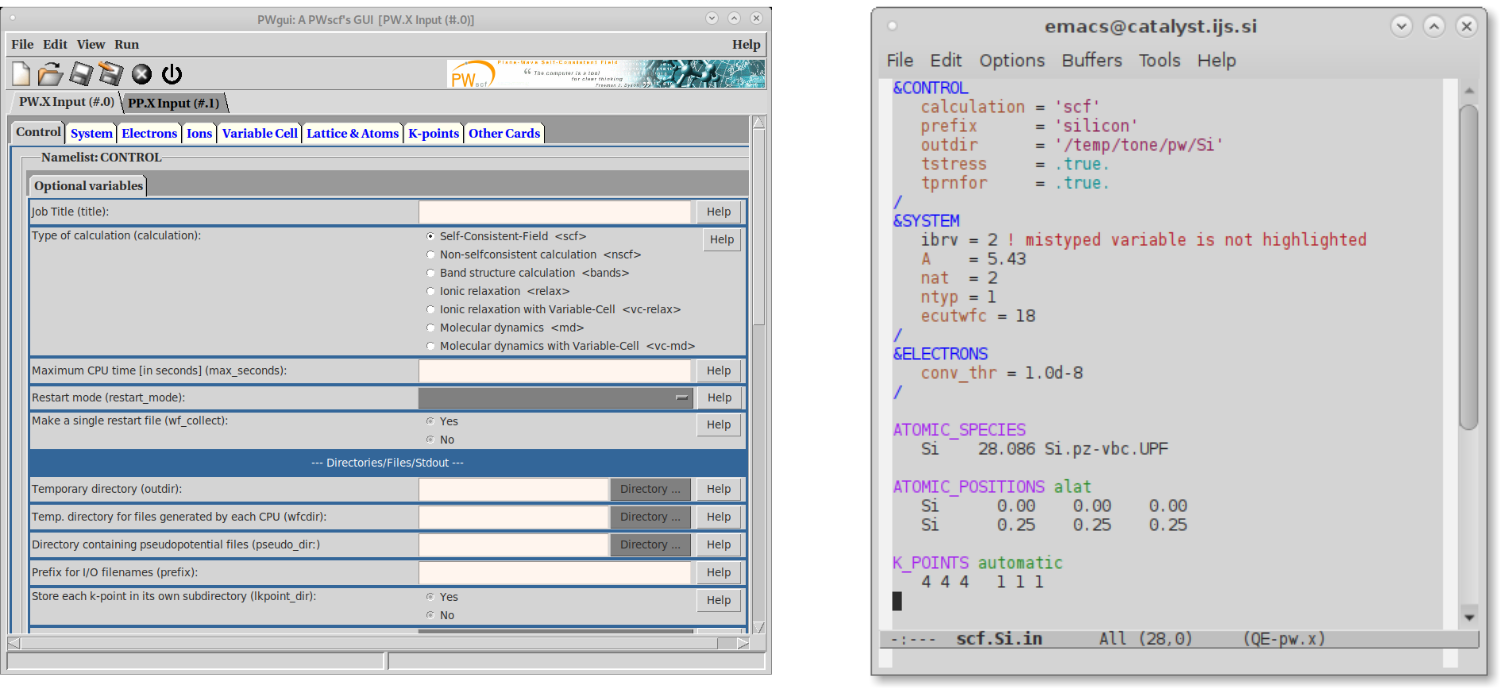
\includegraphics[width=0.8\textwidth]{figs/pwgui+emacs-modes.png}
\end{center}

%%%%%%%%%%%%%%%%%%%%%%%%%%%%%%%%%%%%%%%%%%%%%%%%%%%%%%%%%%%%%
\head{About QE-emacs-modes}
%
\def\bi#1{\textit{\textcolor{blue}{#1}}} \prog{QE-emacs-modes} package
provides syntax highlighting, auto-indentation, and several
utility commands, in particular:
\begin{itemize}
\item[]
  {\small 
    \begin{itemize}
    \item \cmd{Alt-x \bi{prog}-insert-template} -- inserts a respective
      input file template
    \item \cmd{Alt-x \bi{prog-NAMELIST}} -- inserts a blank namelist
      named \bi{NAMELIST}
    \item \cmd{Alt-x \bi{prog-CARD}} -- inserts a blank namelist
      named \bi{CARD}
    \item \cmd{Alt-x \bi{prog-variable}} -- inserts a namelist
      variable named \bi{variable}
    \item \cmd{Alt-x \bi{prog}-mode} -- toggles the respective
      mode
    \item \cmd{Alt-x indent-region} -- indents region
    \end{itemize}
    where
    \begin{itemize}
    \item \cmd{\bi{prog}} is one of \cmd{qe}, \cmd{pw}, \cmd{neb}, \cmd{cp},
      \cmd{ph}, \cmd{ld1}, or \cmd{pp} (these stands for \var{pw.x},
      \var{neb.x}, ... Quantum
      ESPRESSO (QE) programs)
    \item \cmd{\bi{NAMELIST}} is the uppercase name for a given QE namelist
    \item \cmd{\bi{CARD}} is the uppercase name for a given QE card
    \item \cmd{\bi{variable}} is the lowercase name for a given namelist
      variable
    \end{itemize}
  }
\end{itemize}

%%%%%%%%%%%%%%%%%%%%%%%%%%%%%%%%%%%%%%%%%%%%%%%%%%%%%%%%%%%%%
\head{1. How to describe a molecule with Quantum ESPRESSO}
\rightfooter{Example: \file{Day-1/example1.benzene/}}
%
With Quantum ESPRESSO we can describe a molecule by putting it in a
big box.
\begin{center}
  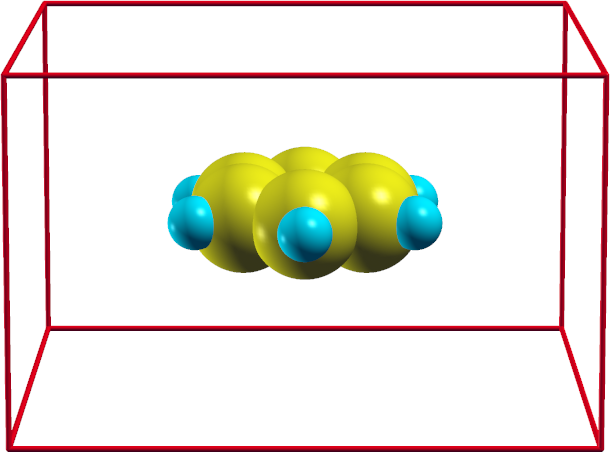
\includegraphics[width=8cm]{figs/benzene-in-box.png}
\end{center}

\begin{itemize}
\item move to \file{Day-1/example1.benzene/} directory
  \vspace{-0.5em}
\item look at the input file \file{pw.benzene.scf.in}. It is composed of three
``namelists'' \nml{\&CONTROL} (note that \var{calculation ='scf'}
is the default value), \nml{\&SYSTEM}, \nml{\&ELECTRONS}, followed 
by three ``cards'' \card{ATOMIC\_SPECIES}, \card{ATOMIC\_POSITIONS},
\card{K\_POINTS}
  \vspace{-0.5em}
\item instructions for how to run the example are in \file{README.md}
\end{itemize}
{\bf Disclaimer:} {\em the box used in this example is very small as to speed-up calculations}

%%%%%%%%%%%%%%%%%%%%%%%%%%%%%%%%%%%%%%%%%%%%%%%%%%%%%%%%%%%%% 
\head{1. How to calculate and plot molecular orbitals}
\rightfooter{Example: \file{Day-1/example1.benzene/}}

Here are the two needed input files for calculation of signed
molecular-orbital densities of benzene (i.e.,
$\sign(\psi_i(\vr))|\psi_i(\vr)|^2$), opened with \prog{emacs} using
\prog{QE-emacs-modes}:
\begin{center}
  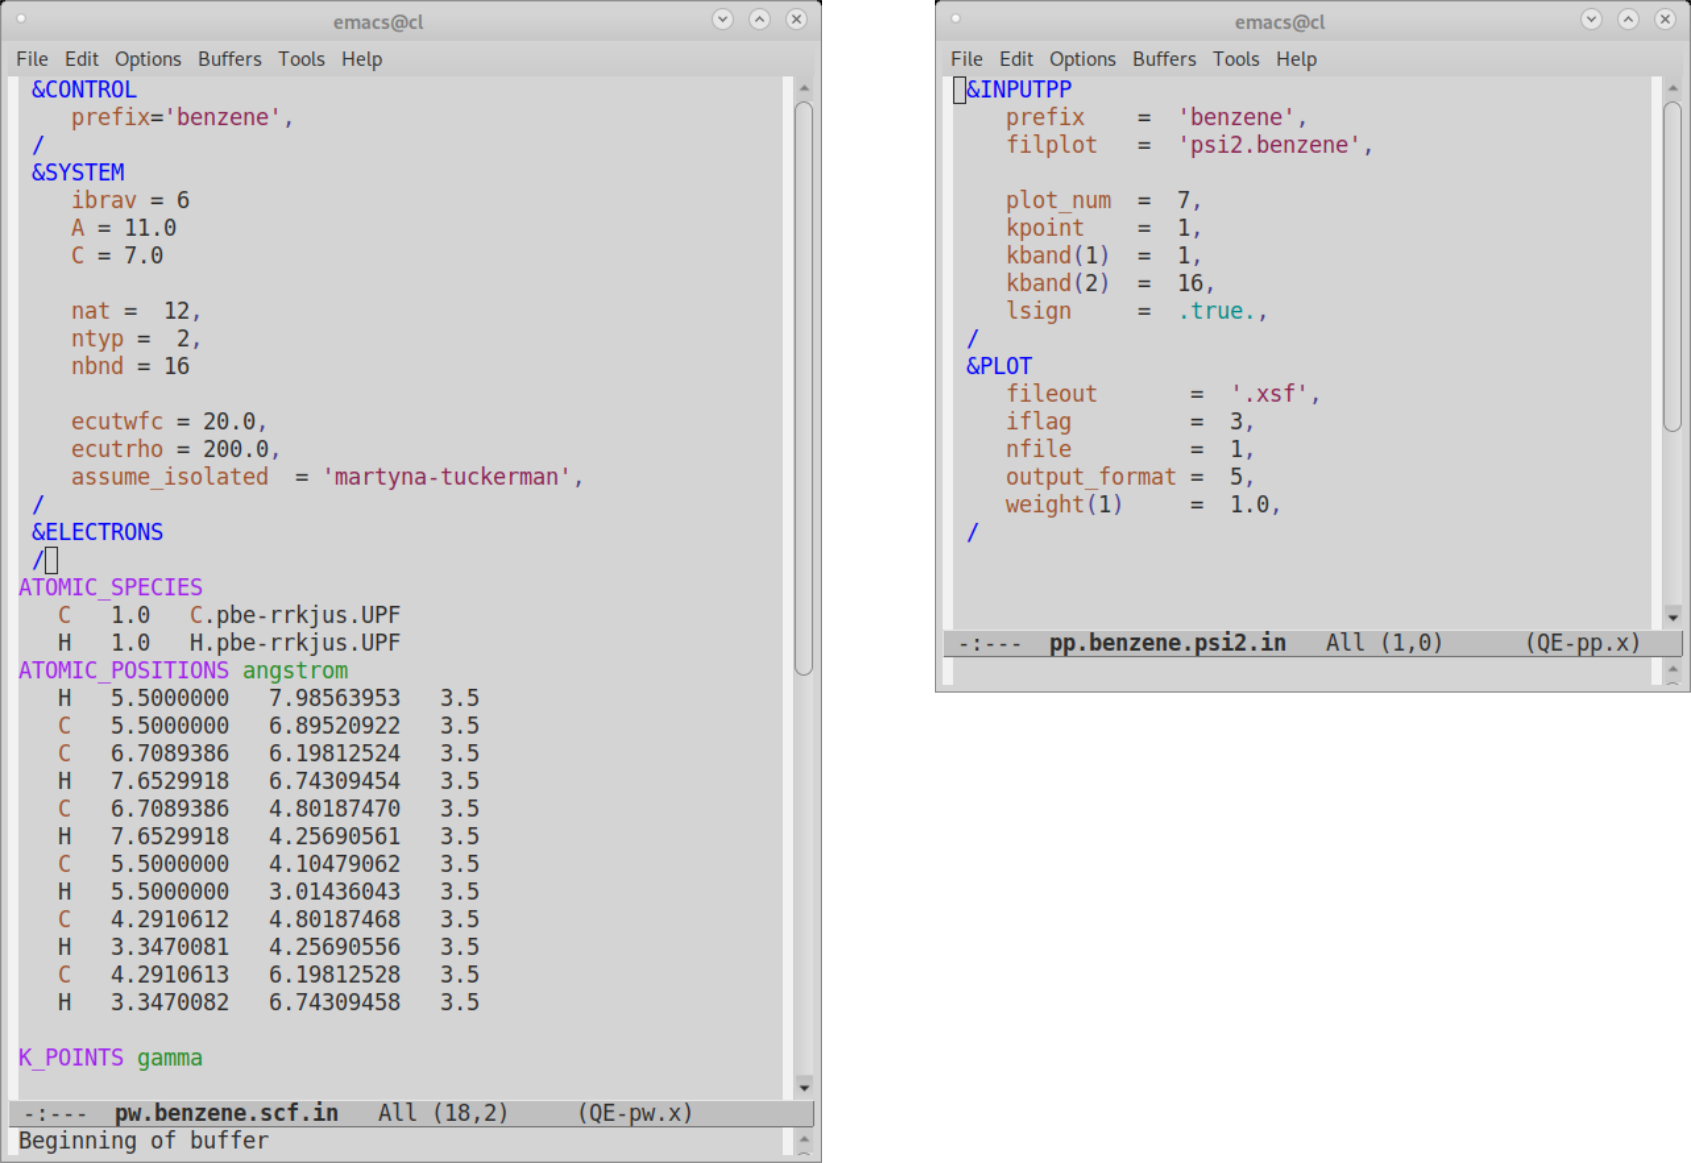
\includegraphics[width=0.8\textwidth]{figs/inputs-benzene.png}
\end{center}

%%%%%%%%%%%%%%%%%%%%%%%%%%%%%%%%%%%%%%%%%%%%%%%%%%%%%%%%%%%%% 
\head{1. How to calculate and plot molecular orbitals}
\rightfooter{Example: \file{Day-1/example1.benzene/}}

To plot signed molecular-orbital densities
($\sign(\psi_i(\vr))|\psi_i(\vr)|^2$), we need to:
\begin{itemize}
\item calculate Kohn-Sham states with \prog{pw.x} (i.e. make an
  SCF calculation)
\item instruct \prog{pp.x} to write them in a suitable format to
  specified files
\item plot orbitals with \prog{xcrysden}
\end{itemize}
See \file{README.md} for detailed instructions.
\vspace{-4cm}
\begin{flushright}
  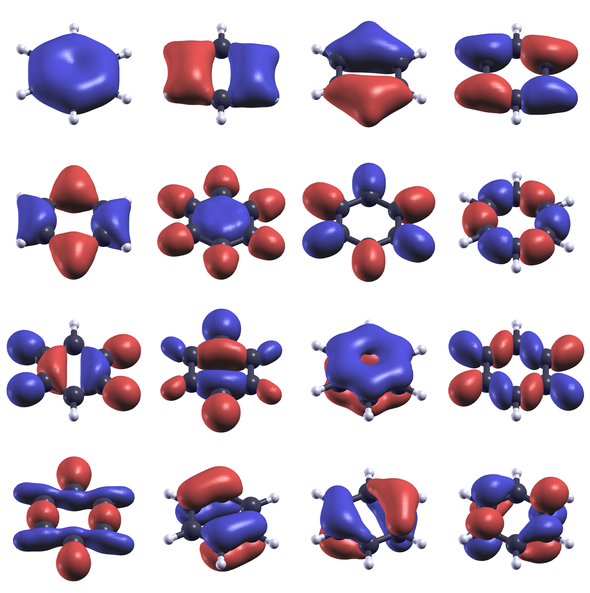
\includegraphics[width=10cm]{figs/psi2-benzene.png}  
\end{flushright}

%%%%%%%%%%%%%%%%%%%%%%%%%%%%%%%%%%%%%%%%%%%%%%%%%%%%%%%%%%%%% 
\head{1. How to plot molecular orbitals with xcrysden}
\rightfooter{Example: \file{Day-1/example1.benzene/}}

\vspace{-0.5em}
\begin{itemize}
\item Execute in the terminal:\\[0.5em]
  %
  \exec{pw.x < pw.benzene.scf.in > pw.benzene.scf.out}\\
  \exec{pp.x < pp.benzene.scf.in > pp.benzene.scf.out}\\[0.5em]
  % 
  {\small The resulting molecular orbitals (i.e., $\sign(\psi(\vr))|\psi(\vr)|^2$) are
  written to \file{psi2.benzene\_*.xsf}}

  \vspace{-0.5em}
\item Plot one of the generated XSF files with \prog{xcrysden},
  e.g.:\\[0.5em]
  % 
  \exec{xcrysden --xsf psi2.benzene\_K001\_B006.xsf}\\[0.5em]
  %
  and follow these instructions:
  \vspace{-0.5em}
  {\small
    \begin{itemize}
    \item use the menu \file{Tools-->Data Grid}; a new window opens, press \file{[OK]}
    \item an isosurface-control window appear; specify the \file{Isovalue},
      say \file{0.005} and press \file{[Submit]}
    \item click the \file{Render +/- isovalue} radiobutton and again
      press \file{[Submit]}
    \item rotate and zoom the structure according to your preference
    \item save the displayed {\em state} via the menu
      \file{File-->Save Current State}\\
      (e.g., save to \file{my-display.xcrysden})
    \item try this with other orbitals, e.g.:\\[0.3em]
      {\small \exec{xcrysden --xsf psi2.benzene\_K001\_B005.xsf --script
          my-display.xcrysden}}
    \end{itemize}
  }
  \vspace{-0.5em}
\item To plot all orbitals, execute: ~\code{./plot-psi2.sh}
\end{itemize}


%%%%%%%%%%%%%%%%%%%%%%%%%%%%%%%%%%%%%%%%%%%%%%%%%%%%%%%%%%%%%
\head{2. How to calculate a 2D-periodic system: graphene}
\rightfooter{Example: \file{Day-1/example2.graphene/}}
%
\parbox{17cm}{A 2D-periodic system (e.g., a graphene sheet) is
  modelled by adding a vacuum layer in the 3rd direction.\\[-0.5em]

  $\bullet$ move to \file{Day-1/example2.graphene/} directory\\[-0.5em]
  
  $\bullet$ look at the input file \file{pw.graphene.scf.in};
  graphene has a 2-atom hexagonal unit cell in the $xy$ plane:
  \var{ibrav=4}, \var{celldm(1)=4.654},\\
  \var{celldm(3)=}\textit{some suitably large value, e.g.} \var{3.0};
}
\hfill \parbox{8cm}{
  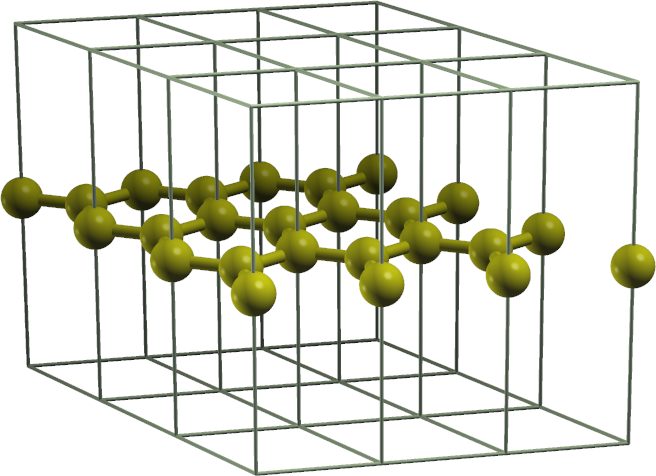
\includegraphics[width=8cm]{figs/graphene.png}\\
}

{\small (remember: \var{celldm(1)} in Bohr radii, \var{celldm(3)=c/a};
  alternatively: \var{A=2.463}, \var{C=7.388} in \AA)}

\parbox{12cm}{
  $\bullet$  atomic positions:\\
\card{
ATOMIC\_POSITIONS (alat)\\
C    0.000000    0.000000    0.000000\\
C    0.000000    0.5773503   0.000000}
}
\hskip 2cm
\parbox{12cm}{
  or, equivalently:\\
  \card{
    ATOMIC\_POSITIONS (crystal)\\
    C    0.000000    0.000000   0.000000\\
    C    0.333333    0.666667   0.000000}
}\\

$\bullet$ k-points: use a dense grid in the $xy$ plane only, e.g.\\
\card{
K\_POINTS (automatic)\\
9 9 1 0 0 0}\\
(a uniform 9$\times$9$\times$1 grid, centered on ${\bf k}=(0,0,0)$ )

%$\bullet$ instructions for how to run the example are in \file{README.md}

%%%%%%%%%%%%%%%%%%%%%%%%%%%%%%%%%%%%%%%%%%%%%%%%%%%%%%%%%%%%%
\head{2. Graphene: DOS and bands (spaghetti)}

\begin{itemize}
\item DOS is typically calculated by a \prog{pw.x} SCF calculation
  followed by a \prog{pw.x} non-SCF calculation (\var{calculation =
    'nscf'}) with a denser k-point grid, and finally using
  \prog{dos.x} post-processing code.

\item to calculate the bands (spaghetti plot), the \prog{pw.x} SCF
  calculation is followed by a \prog{pw.x} ``bands''-type non-SCF
  calculation (\var{calculation = 'bands'}), for which we need a
  suitable path of k-points. The most difficult (?) part is to figure
  out a suitable path of k-points.

  You may either use the ``k-path selection'' tool of \prog{xcrysden}
  or the \prog{SeeK-path} web site at
  \file{http://materialscloud.org/tools/seekpath}.

\item instructions for how to calculate DOS and bands are in \file{README.md}
\end{itemize}

%%%%%%%%%%%%%%%%%%%%%%%%%%%%%%%%%%%%%%%%%%%%%%%%%%%%%%%%%%%%%
\head{K-path selection tool of xcrysden}
~\\[-1.5em]
\centerline{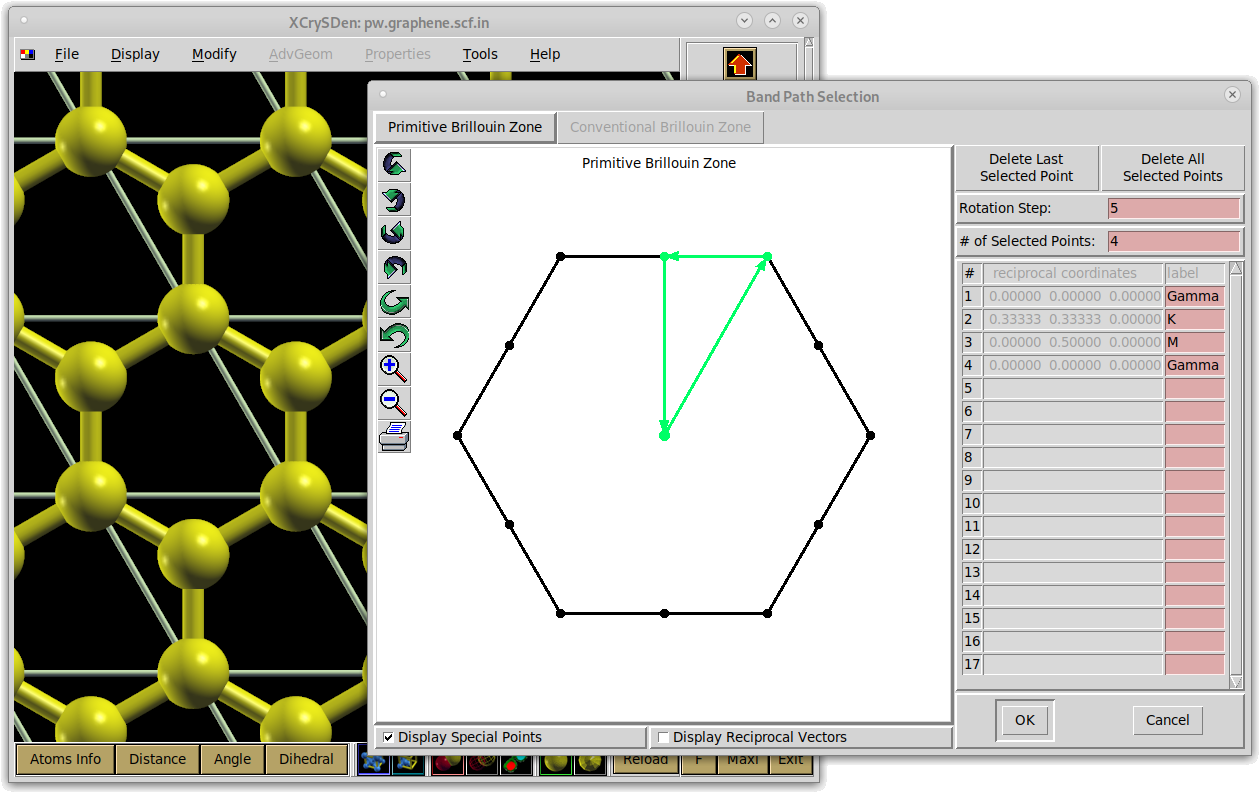
\includegraphics[width=25cm]{figs/xc-k-path.png}}
{\small ({\bf important:} to save k-path in Quantum ESPRESSO format, explicitly
specify the \file{*.pwscf} extension)}

%%%%%%%%%%%%%%%%%%%%%%%%%%%%%%%%%%%%%%%%%%%%%%%%%%%%%%%%%%%%%
\head{SeeK-path @ http://materialscloud.org/tools/seekpath}
~\\
\centerline{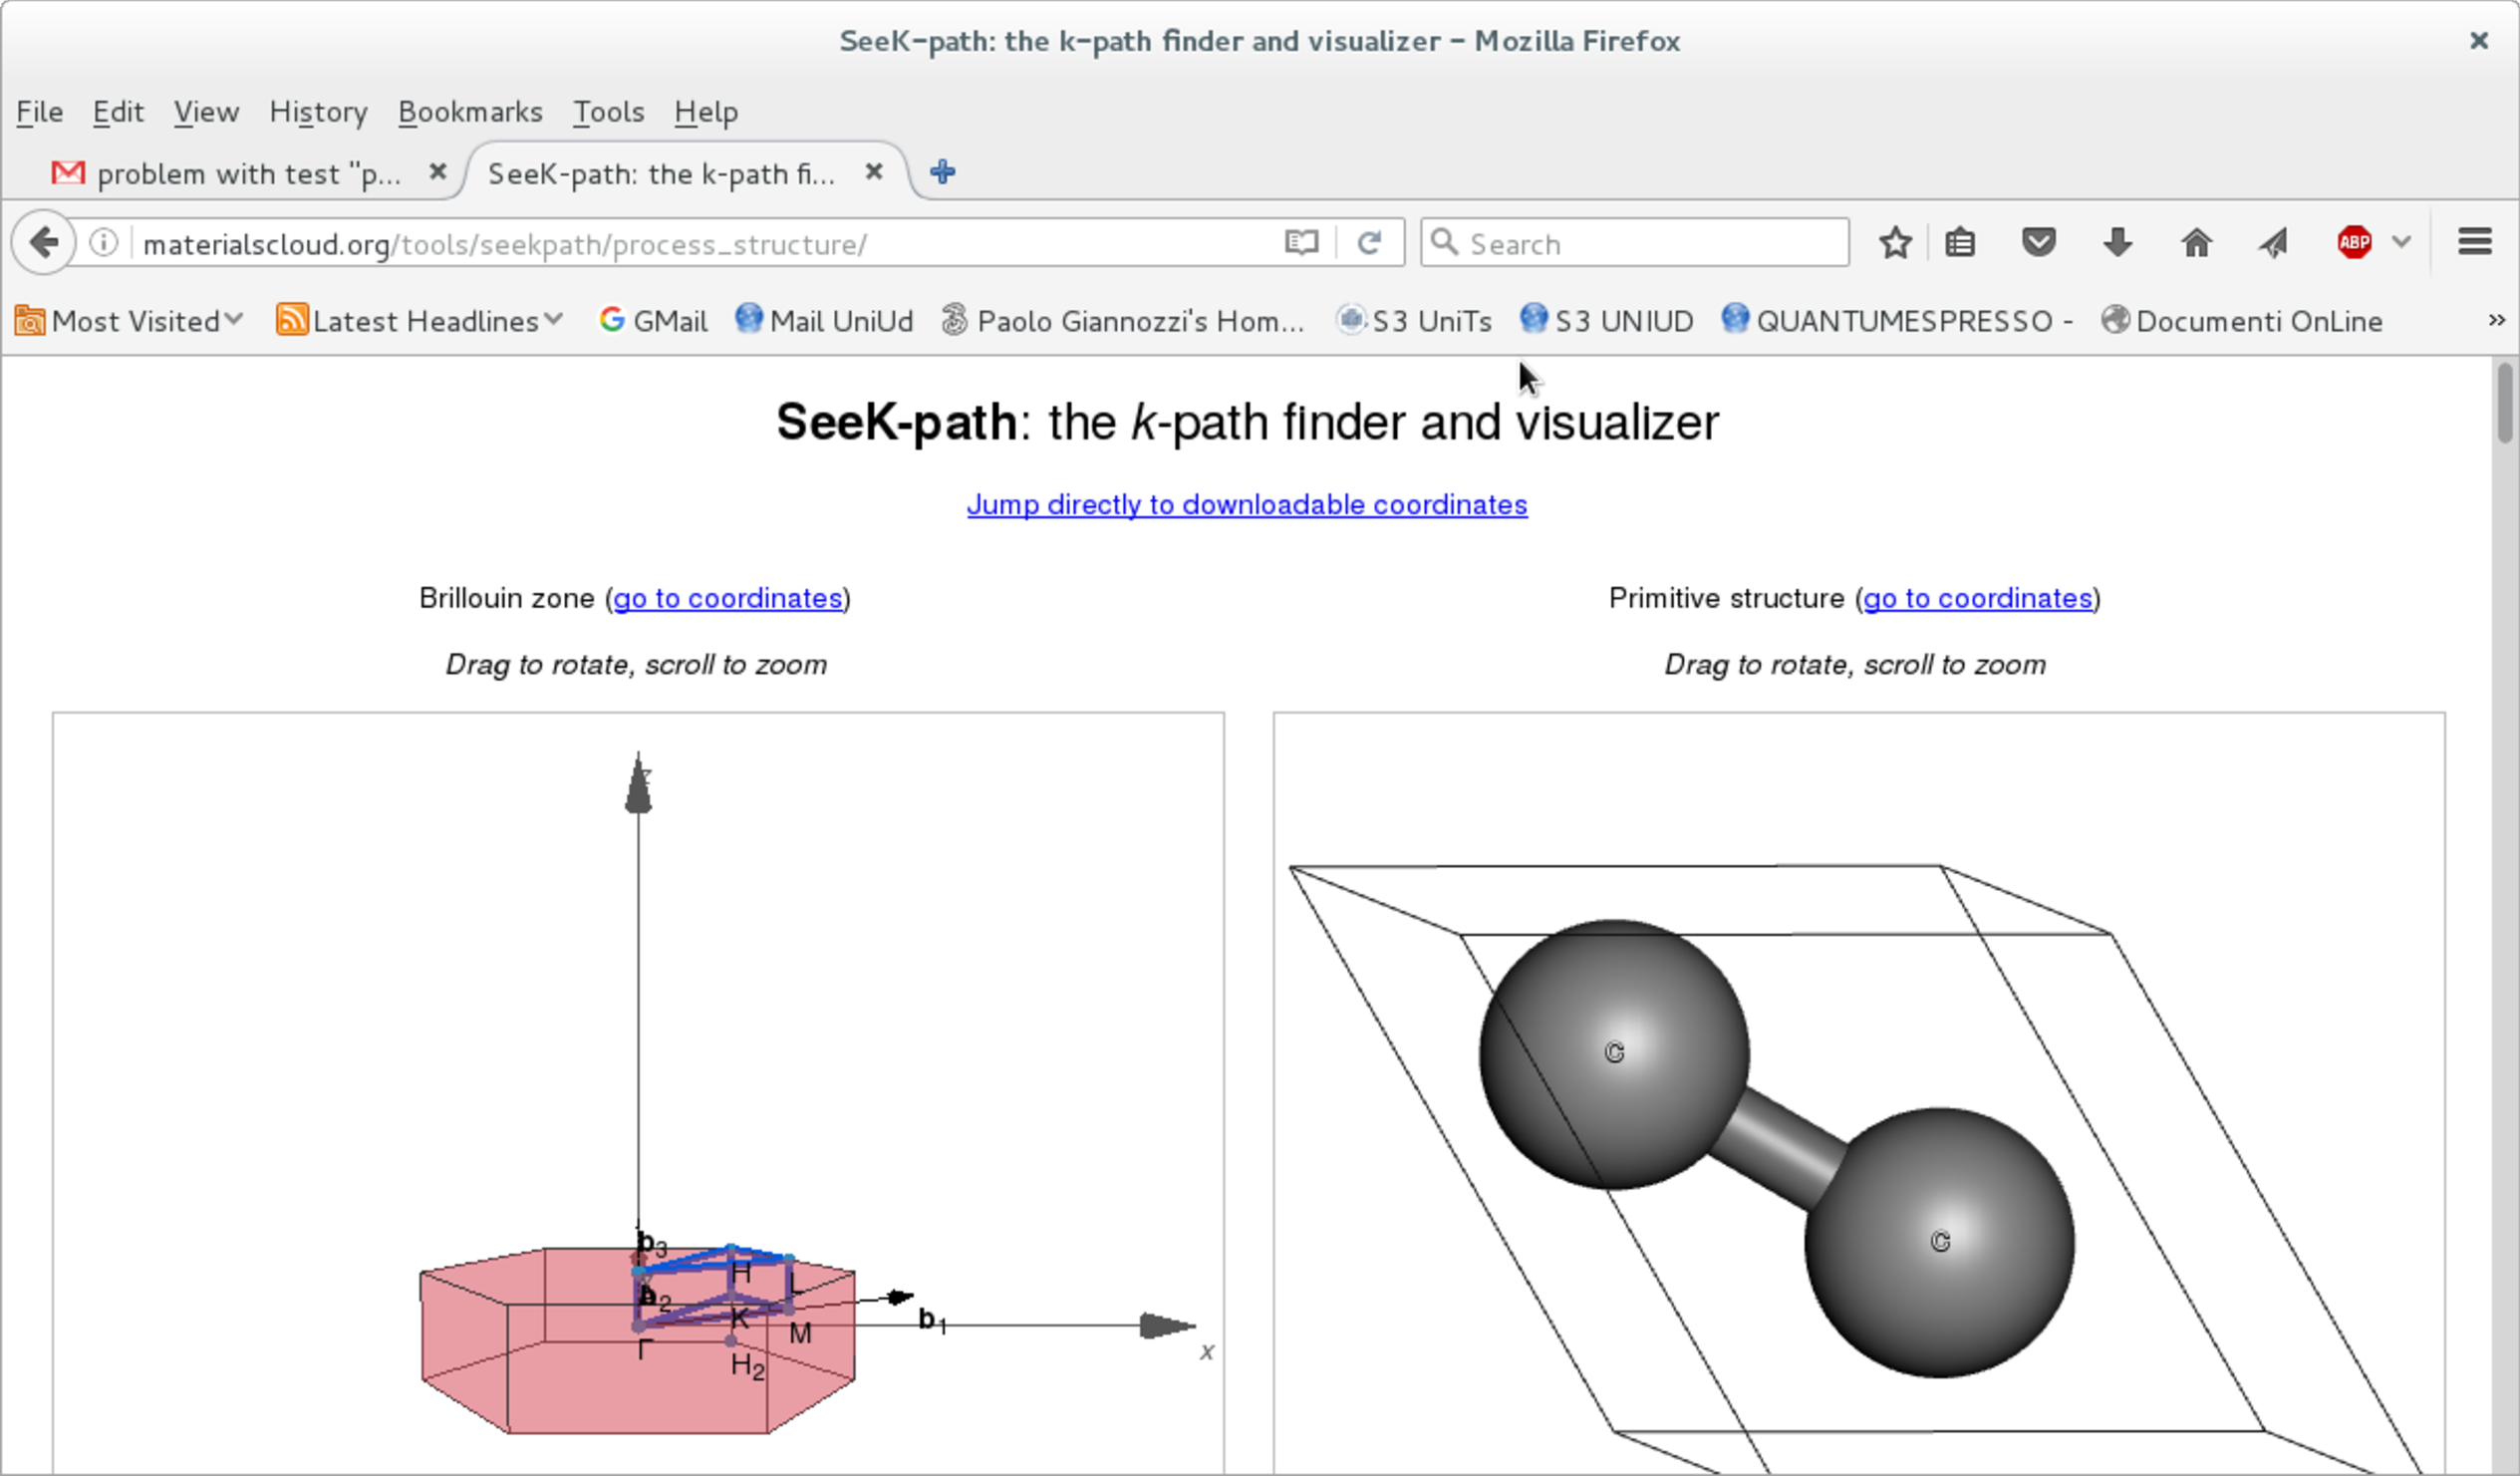
\includegraphics[width=24cm]{figs/seekpath.pdf}}
\end{document}

%%% Local Variables:
%%% mode: latex
%%% TeX-master: t
%%% End:
